\documentclass{../zirkelblatt}
\usepackage{floatflt}
\usepackage{geometry}
\geometry{tmargin=1.5cm,bmargin=1.5cm,lmargin=2cm,rmargin=2cm}

\let\raggedsection\centering
\pagestyle{empty}
\begin{document}

\section*{Satz des Pythagoras}
\begin{floatingfigure}[r]{4cm}
  \vspace{-1cm}
  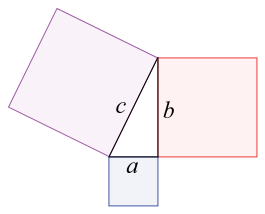
\includegraphics[scale=0.5]{pythagoras-1}
\end{floatingfigure}
Der \emph{Satz des Pythagoras} besagt: Errichtet man auf den drei Kanten eines
rechtwinkligen Dreiecks jeweils ein Quadrat, so sind die beiden kleineren
Quadrate zusammengenommen genauso groß wie das größte Quadrat (siehe Skizze
rechts). Als Formel:
\[ a \cdot a + b \cdot b = c \cdot c. \]
\emph{Wieso ist das so?} Das sollen die beiden anderen Skizzen beantworten.
Kannst du diesen Beweis erklären?
\begin{center}
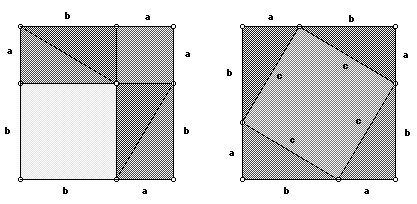
\includegraphics{pythagoras-2}
\end{center}

\vfill

\section*{Summe der natürlichen Zahlen I}
Was ist $1 + 2 + 3 + 4$? Was ist $1 + 2 + 3 + 4 + 5 + 6 + 7 + 8$? Das zu
berechnen, wird immer mühsamer. Zum Glück gibt es eine einfache Formel, die das
Ergebnis sofort liefert:
\begin{align*}
  1 + 2 + 3 + 4 + 5 + 6 + 7 + 8 &= 8 \cdot 9 : 2 \\
  1 + 2 + 3 + 4 + \cdots + 97 + 98 + 99 + 100 &= 100 \cdot 101 : 2
\end{align*}
Die Formel funktioniert auch mit jeder anderen Obergrenze als $100$. \emph{Wieso
stimmt die Formel?} Das soll die Skizze beantworten. Bei ihr ist die
Obergrenze~$6$. Kannst du den Beweis erklären?
\begin{center}
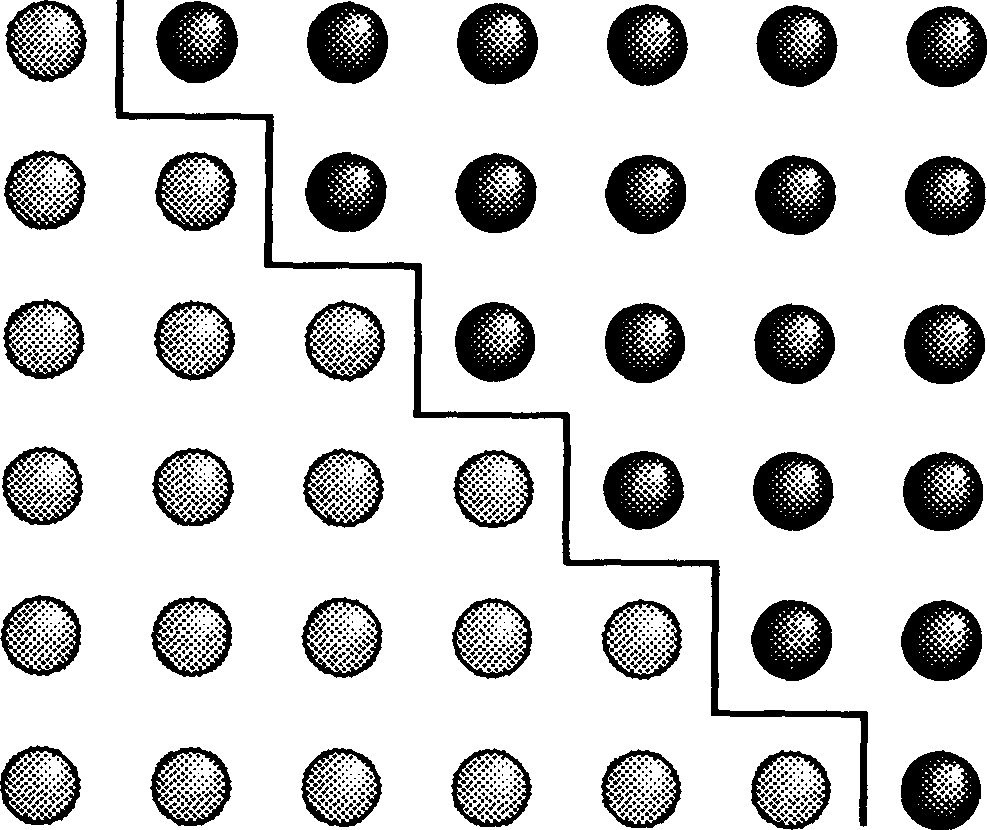
\includegraphics[scale=0.3]{kleiner-gauss-1}
\end{center}


\section*{Summe der natürlichen Zahlen II}
Was ist $1 + 2 + 3 + 4$? Was ist $1 + 2 + 3 + 4 + 5 + 6 + 7 + 8$? Das zu
berechnen, wird immer mühsamer. Zum Glück gibt es eine einfache Formel, die das
Ergebnis sofort liefert:
\begin{align*}
  1 + 2 + 3 + 4 + 5 + 6 + 7 + 8 &= 8 \cdot 9 : 2 \\
  1 + 2 + 3 + 4 + \cdots + 97 + 98 + 99 + 100 &= 100 \cdot 101 : 2
\end{align*}
Die Formel funktioniert auch mit jeder anderen Obergrenze als $100$. \emph{Wieso
stimmt die Formel?} Das soll die Skizze beantworten. Bei ihr ist die
Obergrenze~$100$. Kannst du den Beweis erklären?
\begin{center}
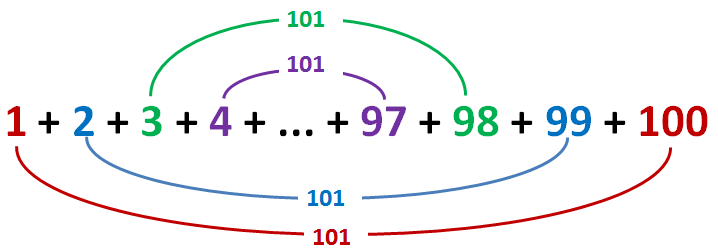
\includegraphics[scale=0.7]{kleiner-gauss-2}
\end{center}


\vfill
\section*{Summe der ungeraden Zahlen}
Was ist $1 + 3 + 5 + 7 + 9$? Was ist $1 + 3 + 5 + 7 + 9 + 11 + 13 + 15$? Das zu
berechnen, wird immer mühsamer. Zum Glück gibt es eine einfache Formel, die das
Ergebnis sofort liefert:
\begin{align*}
  1 + 3 + 5 + 7 + 9 + 11 \phantom{{} + 13 + 15} &= 6 \cdot 6 = 36 \\
  1 + 3 + 5 + 7 + 9 + 11 + 13 \phantom{{} + 15} &= 7 \cdot 7 = 49 \\
  1 + 3 + 5 + 7 + 9 + 11 + 13 + 15 &= 8 \cdot 8 = 64
\end{align*}
\emph{Wieso stimmt die Formel?} Das soll die Skizze beantworten. Kannst du
diesen Beweis erklären?
\begin{center}
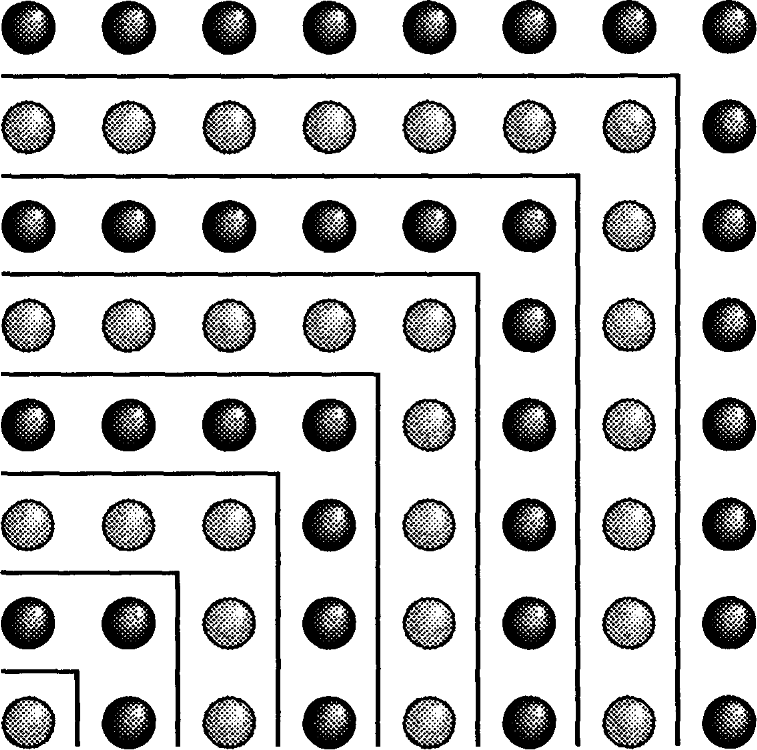
\includegraphics[scale=0.4]{summe-ungerade-zahlen}
\end{center}


\newpage
\section*{Summe der quadrierten Fibonacci-Zahlen}
Bei den \emph{Fibonacci-Zahlen} ergibt die Summe zweier benachbarter Zahlen die
nächste:
\[ 1,\quad 1,\quad 2,\quad 3,\quad 5,\quad 8,\quad 13,\quad 21,\quad 34,\quad 55,\quad 89,\quad \ldots \]
Die \emph{Quadrate} der Fibonacci-Zahlen erfüllen eine interessante Rechenregel:
\begin{align*}
  1\cdot1 \quad+\quad 1\cdot1 \quad+\quad 2\cdot2 \quad+\quad 3\cdot3 \quad+\quad 5\cdot5 \phantom{{} \quad+\quad 8\cdot8 \quad+\quad 13\cdot13}
    &{\quad}=\quad \phantom{0}5 \cdot \phantom{0}8 \\
  1\cdot1 \quad+\quad 1\cdot1 \quad+\quad 2\cdot2 \quad+\quad 3\cdot3 \quad+\quad 5\cdot5 \quad+\quad 8\cdot8 \phantom{{} \quad+\quad 13\cdot13}
    &{\quad}=\quad \phantom{0}8 \cdot 13 \\
  1\cdot1 \quad+\quad 1\cdot1 \quad+\quad 2\cdot2 \quad+\quad 3\cdot3 \quad+\quad 5\cdot5 \quad+\quad 8\cdot8 \quad+\quad 13\cdot13
    &{\quad}=\quad 13 \cdot 21
\end{align*}
Erkennst du das Muster? Wieso die Formeln stimmen, soll die Skizze beweisen.
Kannst du den Beweis erklären?

\emph{Übrigens:} In die Skizze kann man die \emph{goldene Spirale} einzeichnen.
Diese kommt in der Natur an vielen Stellen vor -- hole dir bei mir Beispielbilder ab.
\begin{center}
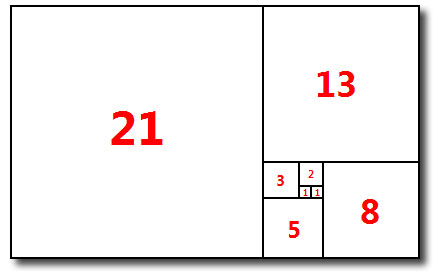
\includegraphics[scale=0.7]{fibonacci-quadrate}
\end{center}

\vfill
\section*{Ein Kästchen verschwindet}
\begin{floatingfigure}[r]{3.5cm}
  \vspace{-0.3cm}
  \scalebox{0.4}{\input{flaecheninhalt-dreieck.pspdftex}}
\end{floatingfigure}
Der Flächeninhalt eines Rechtecks mit den Seitenlängen~$a$ und~$b$ ist~$a \cdot
b$. Der Flächeninhalt eines rechtwinkligen Dreiecks mit Grundseite~$a$ und
Höhe~$h$ ist~$a \cdot h : 2$ (siehe Skizze rechts). Diese beiden Formeln helfen
dir vielleicht für die Aufgabe (oder auch nicht, es gibt mehrere Lösungswege).

In den unteren beiden Skizzen ist irgendwo der Wurm drin. Denn die beiden
Figuren scheinen \emph{denselben Flächeninhalt} zu haben, doch die linke
scheint offensichtlich aus einem Kästchen mehr als die rechte zu bestehen!
Kannst du erklären, was schief läuft?

\begin{center}
  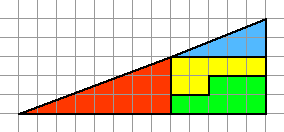
\includegraphics[scale=0.8]{ein-kaestchen-verschwindet-1}
  \hfill
  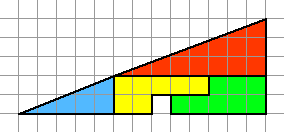
\includegraphics[scale=0.8]{ein-kaestchen-verschwindet-2}
\end{center}


\vfill
\section*{Summe der Dreier-Potenzen}
Für wiederholte Produkte gibt es eine Kurzschreibweise mit \emph{Potenzen}:
\begin{align*}
  5^0 &= 1 \\
  5^1 &= 5 \\
  5^2 &= 5 \cdot 5 = 25 \\
  5^3 &= 5 \cdot 5 \cdot 5 = 125 \\
  5^4 &= 5 \cdot 5 \cdot 5 \cdot 5 = 625 \\\\
  3^7 &= 3 \cdot 3 \cdot 3 \cdot 3 \cdot 3 \cdot 3 \cdot 3
\end{align*}
Was passiert, wenn man die \emph{Dreier-Potenzen} aufsummiert? Dafür gibt es
eine kurze Formel:
\begin{align*}
  3^0 + 3^1 + 3^2 + 3^3 + 3^4 \phantom{{} + 3^5 + 3^6 + 3^7} &= (3^5 - 1) : 2 \\
  3^0 + 3^1 + 3^2 + 3^3 + 3^4 + 3^5 \phantom{{} + 3^6 + 3^7} &= (3^6 - 1) : 2 \\
  3^0 + 3^1 + 3^2 + 3^3 + 3^4 + 3^5 + 3^6 \phantom{{} + 3^7} &= (3^7 - 1) : 2 \\
  3^0 + 3^1 + 3^2 + 3^3 + 3^4 + 3^5 + 3^6 + 3^7 &= (3^8 - 1) : 2
\end{align*}
\emph{Wieso gilt diese Formel?} Das soll die Skizze beweisen. Kannst du den
Beweis erklären?
\begin{center}
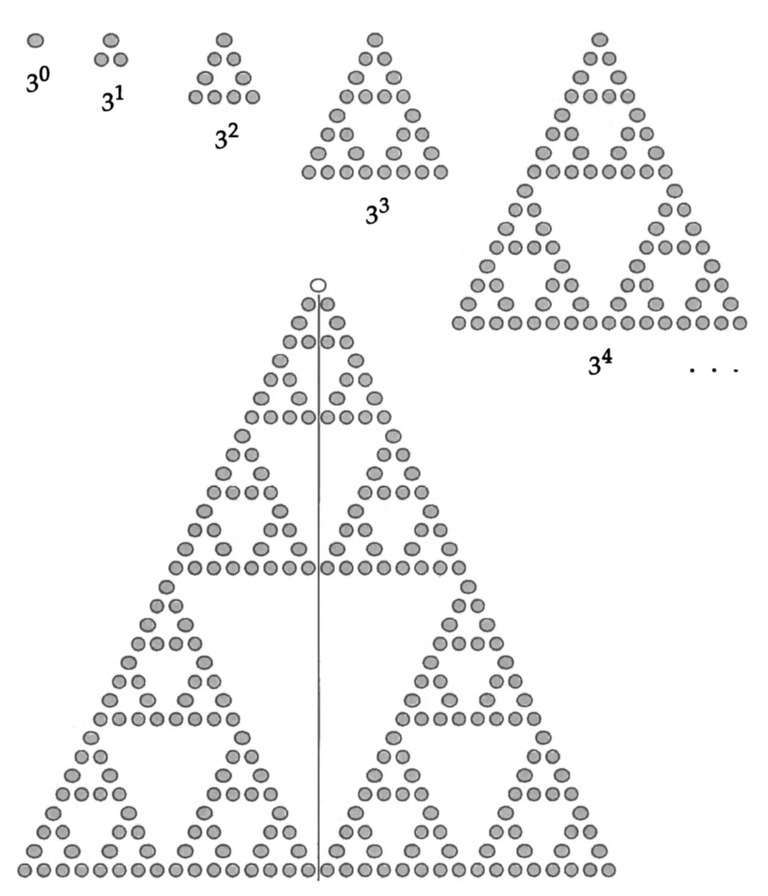
\includegraphics[scale=0.7]{kubikzahlen}
\end{center}


\vfill
\section*{Unendliche Summe der Viertel-Potenzen I}
\emph{Diesen Beweis kann man leider nur verstehen, wenn man bereits Brüche
wie~$\frac{3}{7}$ kennt.}
Den Wert der folgenden unendlichen Reihe kann man
explizit angeben:
\[ \frac{1}{4} + \frac{1}{16} + \frac{1}{64} +
\frac{1}{256} + \frac{1}{1024} + \cdots = \frac{1}{3} \]
Die Skizze soll das beweisen. Kannst du den Beweis erklären?
\begin{center}
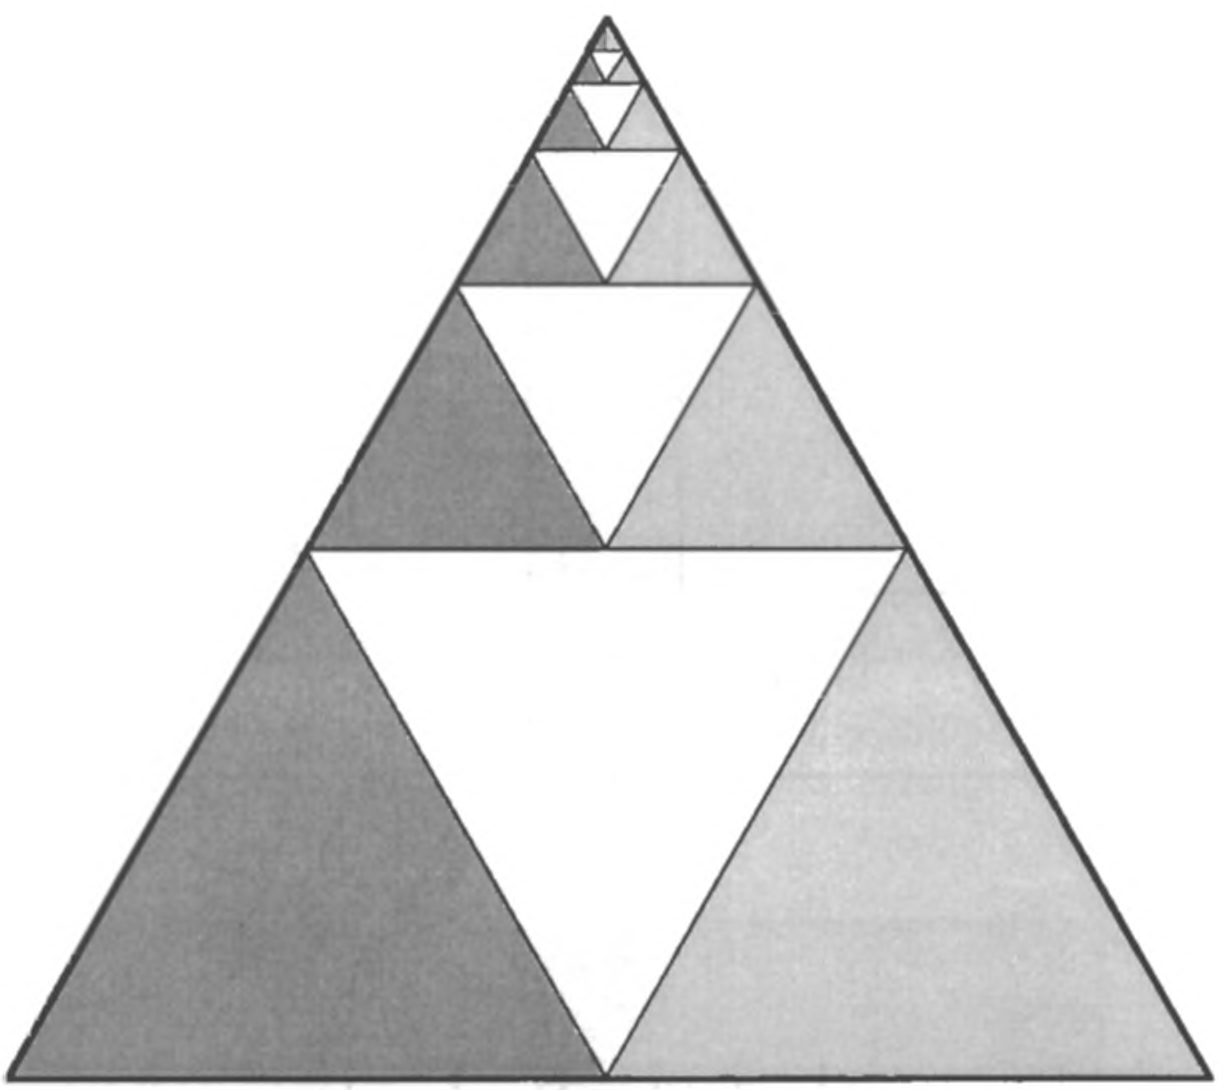
\includegraphics[scale=0.3]{geometrische-reihe-1}
\end{center}


\vfill
\section*{Unendliche Summe der Viertel-Potenzen II}
\emph{Diesen Beweis kann man leider nur verstehen, wenn man bereits Brüche
wie~$\frac{3}{7}$ kennt.}
Den Wert der folgenden unendlichen Reihe kann man
explizit angeben:
\[ \frac{1}{4} + \frac{1}{16} + \frac{1}{64} +
\frac{1}{256} + \frac{1}{1024} + \cdots = \frac{1}{3} \]
Die Skizze soll das beweisen. Kannst du den Beweis erklären?
\begin{center}
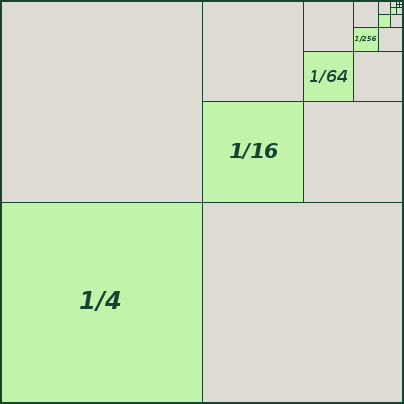
\includegraphics[scale=0.5]{geometrische-reihe-2}
\end{center}


\vfill
\section*{Unendliche Summe der Drittel-Potenzen}
\emph{Diesen Beweis kann man leider nur verstehen, wenn man bereits Brüche
wie~$\frac{3}{7}$ kennt.}
Den Wert der folgenden unendlichen Reihe kann man
explizit angeben:
\[ \frac{1}{3} + \frac{1}{9} + \frac{1}{27} +
\frac{1}{81} + \frac{1}{243} + \cdots = \frac{1}{2} \]
Die Skizze soll das beweisen. Kannst du den Beweis erklären?
\begin{center}
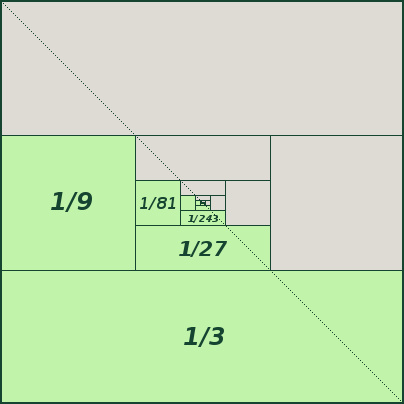
\includegraphics[scale=0.5]{geometrische-reihe-3}
\end{center}


\vfill
\section*{Unendliche Summe der Potenzen von~$\frac{1}{2}$}
\emph{Diesen Beweis kann man leider nur verstehen, wenn man bereits Brüche
wie~$\frac{3}{7}$ kennt.}
Den Wert der folgenden unendlichen Reihe kann man
explizit angeben:
\[ \frac{1}{2} + \frac{1}{4} + \frac{1}{8} +
\frac{1}{16} + \frac{1}{32} + \frac{1}{64} + \cdots = 1 \]
Die Skizze soll das beweisen. Kannst du den Beweis erklären?

\emph{Übrigens:} Im Dualsystem hat die Reihe eine interessante Interpretation. Sie
ist dann analog zur Zahl~$0{,}999\ldots$ im Zehnersystem.
\begin{center}
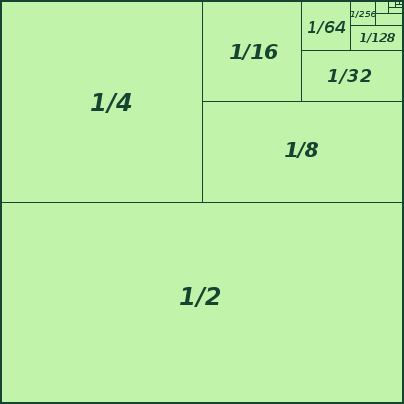
\includegraphics[scale=0.5]{geometrische-reihe-4}
\end{center}


\vfill
\section*{Mersenne-Primzahlen und perfekte Zahlen}
Eine \emph{perfekte Zahl} ist eine Zahl, die gleich der Summe ihrer echten
Teiler ist. Die kleinsten perfekten Zahlen sind~$6$, $28$ und $496$:
\begin{align*}
  6 &= 1 + 2 + 3 \\
  28 &= 1 + 2 + 4 + 7 + 14 \\
  496 &= 1 + 2 + 4 + 8 + 16 + 31 + 62 + 124 + 248
\end{align*}
Bisher hat man nur gerade perfekte Zahlen gefunden. Man weiß noch nicht, ob es
auch ungerade perfekte Zahlen gibt -- das ist ein offenes Forschungsproblem.

Eine \emph{Mersenne-Primzahl} ist eine Primzahl der Form~$2^m-1$. Die ersten
Mersenne-Primzahlen sind:
\begin{align*}
  2^2 - 1 &= 3 \\
  2^3 - 1 &= 7 \\
  2^5 - 1 &= 31 \\
  2^7 - 1 &= 127 \\
  2^{13} - 1 &= 8191
\end{align*}
Es gibt nun folgendes zahlentheoretische Theorem: Ist~$2^{n+1}-1$ eine
Mersenne-Primzahl, so ist die Zahl~$N = 2^n \cdot p$ eine perfekte Zahl. Die
Skizze soll das beweisen. Kannst du den Beweis erklären?
\begin{center}
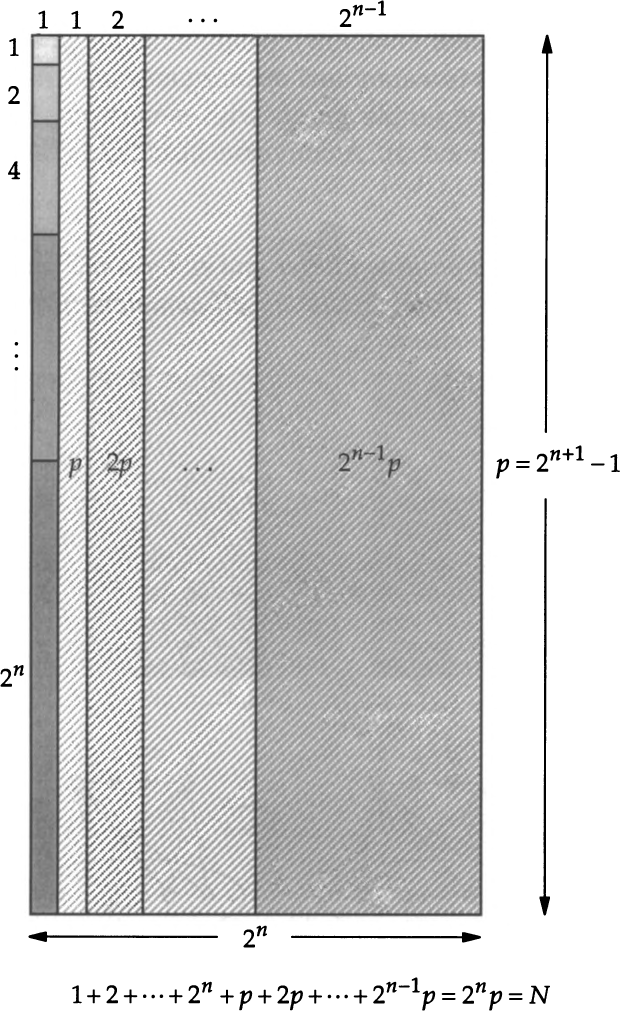
\includegraphics[scale=0.5]{mersenne-perfekt}
\end{center}


\vfill
\section*{Anzahl der Punkte auf Kreis und Gerade}
Ein Kreis hat sicher einen viel kürzeren Umfang als eine unendliche Gerade.
Trotzdem bestehen die beiden Figuren aus \emph{gleich vielen Punkten}! Das soll
die Skizze demonstrieren. Kannst du den Beweis erklären?
\begin{center}
\input{kardinalitaet-kreislinie.pspdftex}
\end{center}

\end{document}

http://upload.wikimedia.org/wikipedia/commons/d/d2/Pythagorean.svg
http://jwilson.coe.uga.edu/EMT668/emt668.student.folders/HeadAngela/essay1/image1.gif
Proofs without Words, Seite 69
http://proofsfromthebook.com/wp-content/uploads/2013/01/sum-of-first-n-positive-integers.png
http://i.stack.imgur.com/QJbdg.jpg
http://i.stack.imgur.com/bLWK1.png
Proofs without Word II, Seite 108
http://3.bp.blogspot.com/_PnLYRqe0k9g/Smp9INIigTI/AAAAAAAAAI0/gQyMxj1hry0/s1600-h/Sum+Of+Fractions+Inverse+Powers+of+4.png
http://4.bp.blogspot.com/_PnLYRqe0k9g/Smpai3DAlBI/AAAAAAAAAIc/7Ornq8sfUvs/s1600-h/Sum+Of+Fractions+Inverse+Powers+of+2.png
Proofs without Word II, Seite 111
